\chapter{Detecting and shifting the bank lines} \label{Chp:BankDetect}

This chapter describes the algorithms used for detecting (see \autoref{Sec:BankDetect}) and shifting (see \autoref{Sec:BankShift}) the bank lines.
The former happens in the 'banklines' step, whereas the latter happens in the 'bankerosion' step after the local bank erosion rate has been computed.

\section{Detecting the bank lines} \label{Sec:BankDetect}

The location of bank lines is determined by looking at the transition of water to land (wet/dry) at a reference discharge computed using \dflowfm.
The detection of the bank lines builds on the search lines provided as input to this step.
The model domain is clipped to the area close to the search lines to focus the bank detection algorithm on the areas of interest only.
The exact location of the bank lines starts by determining for each grid cell in the area of interest whether it has one (or more) bed levels $z_b$ (defined at the mesh nodes) above the water level $z_w$ in the grid cell and one (or more) bed levels below the water level (see \autoref{Fig3.1}).

\Note \dfastbe currently only supports results of hydrodynamic simulations which use bed levels defined at nodes.
Simulations with bed levels defined in cells (tile depth) are thus not supported.

\begin{figure}[!h]
	\vspace{-0.25cm} 
	\center
	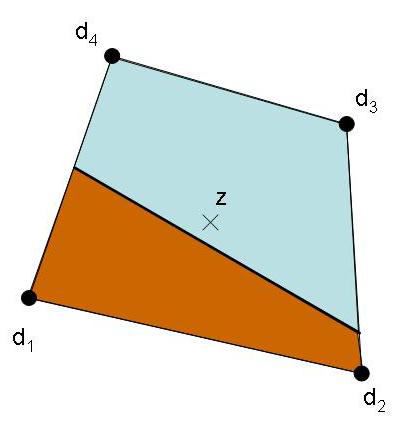
\includegraphics[width=5cm]{figures/Fig3-1.png}
	\caption{The bank line within a transition cell where $d$ equals $z_b$ and $z$ equals $z_w$}
	\label{Fig3.1}
	\vspace{-0.15cm} 
\end{figure}

For each of those grid cells, the subgrid boundary between dry and wet parts is determined as the line along which the interpolated bed level equals the water level in the grid cell.
The line marking the zero water depth is a straight line in a triangle.
Cells with $N_c \ge 4$ corners are split in $N_c - 2$ triangles to arrive at a collection of only straight line segments.
The collection of all these line segments forms the basis of the final bank line.

The found locations of the bank lines will clearlu depend on the chosen discharge level.
However, as long as the discharge is within the main channel, the locations will be fairly consistent.

Generally, bank erosion only occurs along the main channel.
It is therefore possible to only take into account those cells that are within a certain distance from the predefined search lines.
This is also necessary when more than one bank line is present (as is common in rivers), because otherwise it is not clear which coordinates belong to one bank or the other.

The search lines should be defined in a simple text file consisting of x- and y- coordinates (\command{Line1}, ..., \command{LineN}, in the configuration file). For the Dutch rivers the lines can be obained from the Baseline 'oeverlijnen' for model schematisations up to Baseline 4. For modelschematisations of Baseline 5 and higher the oeverlijnen can be obtained by: 1) merging the baseline section 1 and 2 polygon in one polygon feature, 2) transfering this polygon to a polyline feature, 3) cutting this feature into two separate banklines and 4) transforming these lines to points along the lines with an interval of 10 meters.

By using the oeverlijnen, or section 1-2 boundary from Baseline the tool only depicts the main channel. Possible side channels, shortcuts or lakes will not be detected by the tool, see \autoref{Fig3.2}.
If they are important, extra lines should be added that (globally) represent the bank lines of these individual features. For this the input NBank should be increased by the number of extra features and the location of the bank line file \command{LineN} should point to the new file(s) with the xy-coordinates of extra search line(s). It should be noted that for the analysis of these extra bank sections the tool uses the closest point in the mainchannel for which the fairway and riveraxis are specified.

Groynes are not detected as such by the tool, because they are typically defined on subgrid level in the simulations, see \autoref{Fig3.3}.
The detected bank line is in this case following the banks within groyne sections.
This is an advantage, since possible bank erosion only takes place in the groyne sections and not along the groynes themselves.

\begin{figure}[!h]
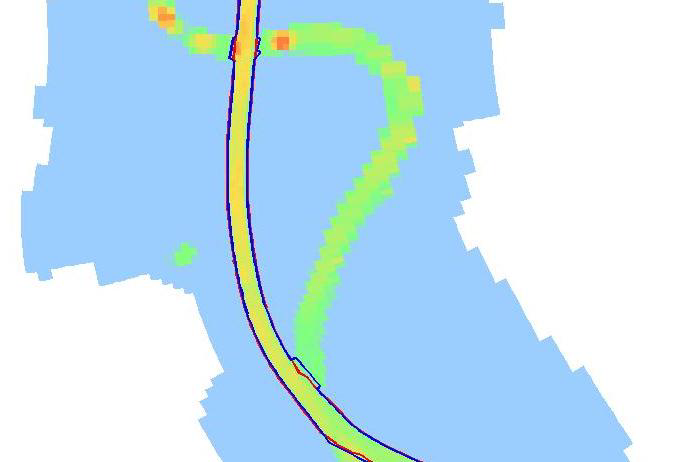
\includegraphics[width=\textwidth,height=7cm]{figures/Fig3-2.png}
\caption{Detection of bank lines at a shortcut in the Meuse river.
Red: Baseline 'section 1-2 boundary', Blue: detected bank line from WAQUA computation (Q = 278.5 m\textsuperscript{3}/s, average discharge)}
\label{Fig3.2}
\end{figure}

\begin{figure}[!hb]
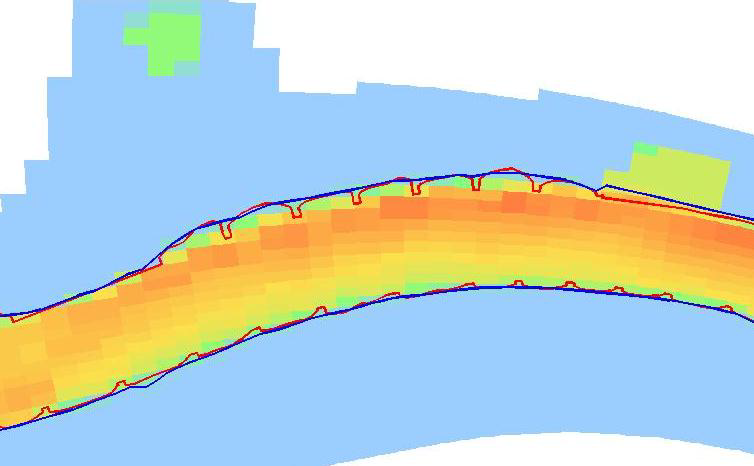
\includegraphics[width=\textwidth,height=7cm]{figures/Fig3-3.png}
\caption{Detection of a bank line close to groynes.
Red: Baseline 'oeverlijnen', Blue: detected bank line from WAQUA computation (Q=278,5 m\textsuperscript{3}/s, average discharge)}
\label{Fig3.3}
\vspace{-0.75cm} 
\end{figure}
\clearpage

\section{Common issues with bank line detection} \label{Sec:DetectIssues}

To be written ...

\emph{`aantal voorbeeld figuren welke aangeven hoe de initi\"ele, door WAQBANK bepaalde oeverlijn gecontroleerd moet worden en hoe de invoer aangepast moet worden om een aantal typische situaties te verbeteren:
•	Oeverlijn van naastgelegen plas/geul/kanaal wordt gevonden: 
o	Op deze locatie meer punten opnemen in de oever invoer welke wordt gebruikt voor het zoeken van de oeverlijn
o	De waterstand voor het bepalen van de oeverligging verlagen
o	Een ander/lager referentieniveau kiezen
o	De afstand/buffer voor de oeverlijnen verkleinen
o	Handmatig een aantal punten verwijderen uit de BankLines uitvoer van WAQBANK voor de oevererosie wordt bepaald door BankErosion (deel 2 van de WAQBANK module) uit te voeren'}

\section{Shifting the bank lines} \label{Sec:BankShift}

The new location of the bank line is determined by shifting each bank line segment individually by its local erosion distance.
In the case of a concave bend the eroding segments move apart; a new bank segment is inserted connecting the two end points of the previously connected segments.
In case of a convex bend the eroding segments overlap; in this case the new bank line follows the outline of furthest erosion.

\begin{figure}[!h]
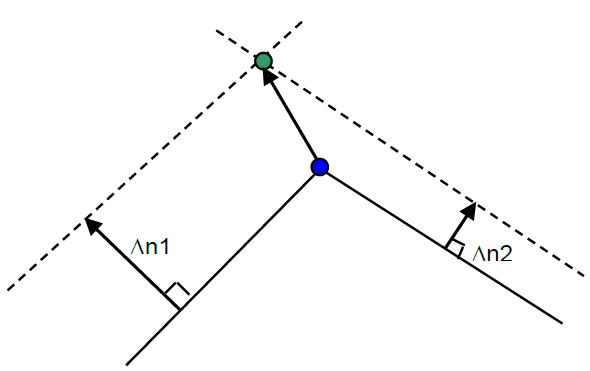
\includegraphics[width=6cm]{figures/Fig4-3.png}
\caption{Het verschuiven van een oeverlijn gebaseerd op het snijpunt van twee lijnsegmenten.
Blauw: oorspronkelijke locatie, Groen: nieuwe locatie}
\label{Fig4.3}
\end{figure}

\begin{figure}[!h]
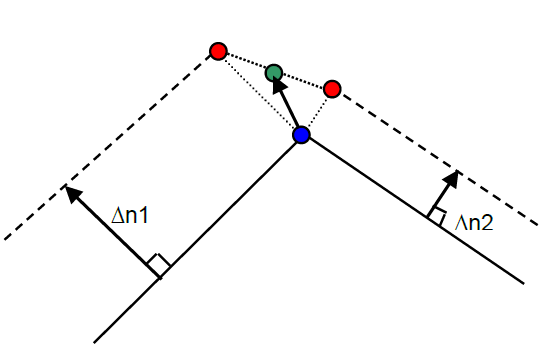
\includegraphics[width=5cm]{figures/Fig4-4.png}
\caption{Het verschuiven van een oeverlijn gebaseerd op de gemiddelde verplaatsing van twee lijnsegmenten.
Blauw: oorspronkelijke locatie, Rood: nieuwe locatie gebaseerd op individuele segmenten, Groen: nieuwe locatie (gemiddelde van de rode punten).}
\label{Fig4.4}
\end{figure}